
\section{Paradigma No 01 – Programación Imperativa} 

\begin{enumerate}[1.]
	\item La Programación Imperativa  es una paradigma de programación imperativa al lenguaje de programación como tiene que realizar cada uno de los pasos. Le decimos que variables usar, que bucles y sentencias etc. Es decir, construimos un algoritmo muy concreto para solventar un problema\\
\textbf{Nociones Básicas:}
\item Variable con estado (valor modificable)
\item Secuencia de cambios de estado
\item Procedimientos 
\textbf{Características Destacables:}
\item Se fija completamente el orden en el que se deben realizar las operaciones con ayuda de unos patrones de control del flujo de ejecución (secuencia, alternativa y ciclo) que sirven para construir el esqueleto de las rutinas.

\item Se pueden fijar puntos de observación en el texto de una rutina y considerar los valores de las variables (estado) cuando el flujo de ejecución pasa por dichos puntos. Estos valores pueden cambiar de un punto a otro y en el mismo punto en momentos distintos de la ejecución. 


\textbf{Estructuras Cíclicas de Control:}
La mayoría de lenguajes de programación imperativos tienen estructuras cíclicas de control tales como while, do..while, for y loop para iterar sobre un determinado bloque de códigos dada una condición o expresión, mientras que la gran mayoría de lenguajes declarativos, especialmente los funcionales (subparadigma declarativo), carecen de este tipo de estructuras cíclicas, de hecho la única forma de representar un flujo cíclico es a través de la recursión (funciones que se llaman a sí misma) o través de funciones de alto nivel tales como map y reduce (que internamente usan recursión).

\textbf{Procedimiento:}
\item Secuencia de actuaciones sobre el estado de ciertas variables para alcanzar unos valores que cumplan unas determinadas condiciones. Tienen nombre y parámetros (de entrada y de salida).
\item Los procedimientos colaboran pasando valores de los parámetros de salida de unos a los parámetros de entrada de otros.

\textbf{Estructura de Datos:}
\item Datos predefinidos (v. lógicos, números, caracteres)
\item Esquemas de array, de registro y variables dinámicas

	

\end{enumerate}

\section{Paradigma No 02 – Programación Orientada a Objetos} 

\begin{enumerate}[1.]
	\item definición Programación orientada a objetos (POO)\\

Es un paradigma de programación que usa objetos y sus interacciones, para diseñar aplicaciones y programas informáticos. Está basado en varias técnicas, incluyendo herencia, abstracción, polimorfismo y encapsulamiento. Su uso se popularizó a principios de la década de los años 1990. En la actualidad, existe variedad de lenguajes de programación que soportan la orientación a objetos.\\
{enumerate}[2.]
\item \textbf{Introduccion:}\\

Los objetos son entidades que combinan estado (atributo), comportamiento (método) e identidad:\\

\textbf{El estado(atributo):}\\

Está compuesto de datos, será uno o varios atributos a los que se habrán asignado unos valores concretos (datos).

\textbf{El comportamiento(métodos):}\\

está definido por los procedimientos o métodos con que puede operar dicho objeto, es decir, qué operaciones se pueden realizar con él.\\

\textbf{La identidad(identificadores):}\\

Es una propiedad de un objeto que lo diferencia del resto, dicho con otras palabras, es su identificador (concepto análogo al de identificador de una variable o una constante).
Un objeto contiene toda la información que permite definirlo e identificarlo frente a otros objetos pertenecientes a otras clases e incluso frente a objetos de una misma clase, al poder tener valores bien diferenciados en sus atributos. A su vez, los objetos disponen de mecanismos de interacción llamados métodos, que favorecen la comunicación entre ellos. Esta comunicación favorece a su vez el cambio de estado en los propios objetos. Esta característica lleva a tratarlos como unidades indivisibles, en las que no se separa el estado y el comportamiento.
Los métodos (comportamiento) y atributos (estado) están estrechamente relacionados por la propiedad de conjunto. Esta propiedad destaca que una clase requiere de métodos para poder tratar los atributos con los que cuenta. El programador debe pensar indistintamente en ambos conceptos, sin separar ni darle mayor importancia a alguno de ellos. Hacerlo podría producir el hábito erróneo de crear clases contenedoras de información por un lado y clases con métodos que manejen a las primeras por el otro. De esta manera se estaría realizando una programación estructurada camuflada en un lenguaje de programación orientado a objetos.
La POO difiere de la programación estructurada tradicional, en la que los datos y los procedimientos están separados y sin relación, ya que lo único que se busca es el procesamiento de unos datos de entrada para obtener otros de salida. La programación estructurada anima al programador a pensar sobre todo en términos de procedimientos o funciones, y en segundo lugar en las estructuras de datos que esos procedimientos manejan. En la programación estructurada sólo se escriben funciones que procesan datos. Los programadores que emplean POO, en cambio, primero definen objetos para luego enviarles mensajes solicitándoles que realicen sus métodos por sí mismos.\\
{enumerate}[3.]
\item \textbf{Origen:}\\

Los conceptos de la programación orientada a objetos tienen origen en Simula 67, un lenguaje diseñado para hacer simulaciones, creado por Ole-Johan Dahl y Kristen Nygaard del Centro de Cómputo Noruego en Oslo. En este centro, se trabajaba en simulaciones de naves, que fueron confundidas por la explosión combinatoria de cómo las diversas cualidades de diferentes naves podían afectar unas a las otras. La idea ocurrió para agrupar los diversos tipos de naves en diversas clases de objetos, siendo responsable cada clase de objetos de definir sus propios datos y comportamientos. Fueron refinados más tarde en Smalltalk, que fue desarrollado en Simula en Xerox PARC (cuya primera versión fue escrita sobre Basic) pero diseñado para ser un sistema completamente dinámico en el cual los objetos se podrían crear y modificar "en marcha" (en tiempo de ejecución) en lugar de tener un sistema basado en programas estáticos.
La programación orientada a objetos tomó posición como el estilo de programación dominante a mediados de los años ochenta, en gran parte debido a la influencia de C++, una extensión del lenguaje de programación C. Su dominación fue consolidada gracias al auge de las Interfaces gráficas de usuario, para las cuales la programación orientada a objetos está particularmente bien adaptada. En este caso, se habla también de programación dirigida por eventos.
Las características de orientación a objetos fueron agregadas a muchos lenguajes existentes durante ese tiempo, incluyendo Ada, BASIC, Lisp, Pascal, entre otros. La adición de estas características a los lenguajes que no fueron diseñados inicialmente para ellas condujo a menudo a problemas de compatibilidad y en la capacidad de mantenimiento del código. Los lenguajes orientados a objetos "puros", por su parte, carecían de las características de las cuales muchos programadores habían venido a depender. Para saltar este obstáculo, se hicieron muchas tentativas para crear nuevos lenguajes basados en métodos orientados a objetos, pero permitiendo algunas características imperativas de maneras "seguras". El Eiffel de Bertrand Meyer fue un temprano y moderadamente acertado lenguaje con esos objetivos pero ahora ha sido esencialmente reemplazado por Java, en gran parte debido a la aparición de Internet, y a la implementación de la máquina virtual de Java en la mayoría de navegadores. PHPen su versión 5 se ha modificado, soporta una orientación completa a objetos, cumpliendo todas las características propias de la orientación a objetos.\\
{enumerate}[4.]
\item \textbf{Conceptos Fundamentales:}\\

La programación orientada a objetos es una forma de programar que trata de encontrar una solución a estos problemas. Introduce nuevos conceptos, que superan y amplían conceptos antiguos ya conocidos. Entre ellos destacan los siguientes:\\

\textbf{Clase:}\\

Definiciones de las propiedades y comportamiento de un tipo de objeto concreto. La instanciación es la lectura de estas definiciones y la creación de un objeto a partir de ellas.\\

\textbf{Herencia:}\\

Es la facilidad mediante la cual la clase D hereda en ella cada uno de los atributos y operaciones de C, como si esos atributos y operaciones hubiesen sido definidos por la misma D. Por lo tanto, puede usar los mismos métodos y variables publicas declaradas en C. Los componentes registrados como "privados" (private) también se heredan, pero como no pertenecen a la clase, se mantienen escondidos al programador y sólo pueden ser accedidos a través de otros métodos públicos. Esto es así para mantener hegemónico el ideal de OOP.\\

\textbf{Objeto:}\\

Entidad provista de un conjunto de propiedades o atributos (datos) y de comportamiento o funcionalidad (métodos) los mismos que consecuentemente reaccionan a eventos. Se corresponde con los objetos reales del mundo que nos rodea, o a objetos internos del sistema (del programa). Es una instancia a una clase.\\


\textbf{Metodo:}\\

Algoritmo asociado a un objeto (o a una clase de objetos), cuya ejecución se desencadena tras la recepción de un "mensaje". Desde el punto de vista del comportamiento, es lo que el objeto puede hacer. Un método puede producir un cambio en las propiedades del objeto, o la generación de un "evento" con un nuevo mensaje para otro objeto del sistema.\\


\textbf{Evento:}\\

Es un suceso en el sistema (tal como una interacción del usuario con la máquina, o un mensaje enviado por un objeto). El sistema maneja el evento enviando el mensaje adecuado al objeto pertinente. También se puede definir como evento, a la reacción que puede desencadenar un objeto, es decir la acción que genera.\\


\textbf{Mensaje:}\\

Una comunicación dirigida a un objeto, que le ordena que ejecute uno de sus métodos con ciertos parámetros asociados al evento que lo generó.\\


\textbf{Propiedad o Atributo:}\\

Contenedor de un tipo de datos asociados a un objeto (o a una clase de objetos), que hace los datos visibles desde fuera del objeto y esto se define como sus características predeterminadas, y cuyo valor puede ser alterado por la ejecución de algún método.\\


\textbf{Estado Interno:}\\

Es una variable que se declara privada, que puede ser únicamente accedida y alterada por un método del objeto, y que se utiliza para indicar distintas situaciones posibles para el objeto (o clase de objetos). No es visible al programador que maneja una instancia de la clase.\\


\textbf{Componentes de un Objeto:}\\

Atributos, identidad, relaciones y métodos.\\


\textbf{Identificacion de un Objeto:}\\

Un objeto se representa por medio de una tabla o entidad que esté compuesta por sus atributos y funciones correspondientes.
En comparación con un lenguaje imperativo, una "variable", no es más que un contenedor interno del atributo del objeto o de un estado interno, así como la "función" es un procedimiento interno del método del objeto.\\


{enumerate}[5.]
\item \textbf{Caracteristicas de la POO:}\\

Existe un acuerdo acerca de qué características contempla la "orientación a objetos", las características siguientes son las más importantes:\\

\textbf{Abstraccion:}\\

Denota las características esenciales de un objeto, donde se capturan sus comportamientos.Cada objeto en el sistema sirve como modelo de un "agente" abstracto que puede realizar trabajo, informar y cambiar su estado, y "comunicarse" con otros objetos en el sistema sin revelar cómo se implementan estas características. Los procesos, las funciones o los métodos pueden también ser abstraídos y cuando lo están, una variedad de técnicas son requeridas para ampliar una abstracción.El proceso de abstracción permite seleccionar las características relevantes dentro de un conjunto e identificar comportamientos comunes para definir nuevos tipos de entidades en el mundo real. La abstracción es clave en el proceso de análisis y diseño orientado a objetos, ya que mediante ella podemos llegar a armar un conjunto de clases que permitan modelar la realidad o el problema que se quiere atacar.\\

\textbf{Encapsulamiento:}\\

Significa reunir a todos los elementos que pueden considerarse pertenecientes a una misma entidad, al mismo nivel de abstracción. Esto permite aumentar la cohesión de los componentes del sistema. Algunos autores confunden este concepto con el principio de ocultación, principalmente porque se suelen emplear conjuntamente.\\


\textbf{Principio de Ocultacion:}\\

Cada objeto está aislado del exterior, es un módulo natural, y cada tipo de objeto expone una interfaz a otros objetos que especifica cómo pueden interactuar con los objetos de la clase. El aislamiento protege a las propiedades de un objeto contra su modificación por quien no tenga derecho a acceder a ellas, solamente los propios métodos internos del objeto pueden acceder a su estado. Esto asegura que otros objetos no pueden cambiar el estado interno de un objeto de maneras inesperadas, eliminando efectos secundarios e interacciones inesperadas. Algunos lenguajes relajan esto, permitiendo un acceso directo a los datos internos del objeto de una manera controlada y limitando el grado de abstracción. La aplicación entera se reduce a un agregado o rompecabezas de objetos.\\


\textbf{Polimorfismo:}\\

Comportamientos diferentes, asociados a objetos distintos, pueden compartir el mismo nombre, al llamarlos por ese nombre se utilizará el comportamiento correspondiente al objeto que se esté usando. O dicho de otro modo, las referencias y las colecciones de objetos pueden contener objetos de diferentes tipos, y la invocación de un comportamiento en una referencia producirá el comportamiento correcto para el tipo real del objeto referenciado. Cuando esto ocurre en "tiempo de ejecución", esta última característica se llama asignación tardía o asignación dinámica. Algunos lenguajes proporcionan medios más estáticos (en "tiempo de compilación") de polimorfismo, tales como las plantillas y la sobrecarga de operadores de C++.\\

\textbf{Herencia:}\\

Las clases no están aisladas, sino que se relacionan entre sí, formando una jerarquía de clasificación. Los objetos heredan las propiedades y el comportamiento de todas las clases a las que pertenecen. La herencia organiza y facilita el polimorfismo y el encapsulamiento permitiendo a los objetos ser definidos y creados como tipos especializados de objetos preexistentes. Estos pueden compartir (y extender) su comportamiento sin tener que volver a implementarlo. Esto suele hacerse habitualmente agrupando los objetos en clases y estas en árboles o enrejados que reflejan un comportamiento común. Cuando un objeto hereda de más de una clase se dice que hay herencia múltiple.\\


\textbf{Recoleccion de Basura:}\\

La recolección de basura o garbage collector es la técnica por la cual el entorno de objetos se encarga de destruir automáticamente, y por tanto desvincular la memoria asociada, los objetos que hayan quedado sin ninguna referencia a ellos. Esto significa que el programador no debe preocuparse por la asignación o liberación de memoria, ya que el entorno la asignará al crear un nuevo objeto y la liberará cuando nadie lo esté usando. En la mayoría de los lenguajes híbridos que se extendieron para soportar el Paradigma de Programación Orientada a Objetos como C++ u Object Pascal, esta característica no existe y la memoria debe desasignarse manualmente.\\


\textbf{Entre los lenguajes orientados a objetos se destacan los siguientes:}\\

\begin {itemize}
\item ABAP
\item ActionScript
\item C++
\item CSharp
\item Java
\item JavaScript (la herencia se realiza por medio de la programación basada en prototipos)
\item Perl (soporta herencia múltiple. La resolución se realiza en preorden, pero puede modificarse al algoritmo linearization C3 por medio del módulo Class::C3 en CPAN)
\item PHP (a partir de su versión 5)
\item PowerBuilder
\item Python
\item Ruby
\end{itemize}









\end{enumerate}



\section{Paradigma No 03 – Programación Lógico} 

\begin{enumerate}[1.]
	\item La Programación Lógica  
¿Qué es?
La programación lógica es un paradigma que se encuentra dentro del paradigma de la programación funcional. Aunque no es tan conocido como otros paradigmas de programación, es realmente interesante. Se basa en la declaración de hechos y reglas que permiten ir creando lo que para nosotros sería el conocimiento. Aunque inicialmente sea un poco complejo de entender, la programación lógica trabaja de forma muy similar a los humanos en cuanto al manejo de información y conocimientos se refiere. Veamos un ejemplo para entender mejor cómo es la declaración de las reglas y hechos
Paradigma de programación basado en la lógica de primer orden. La Programación Lógica estudia el uso de la lógica para el planteamiento de problemas y el control sobre las reglas de inferencia para alcanzar la solución automática.
La Programación Lógica, junto con la funcional, forma parte de lo que se conoce como Programación Declarativa, es decir la programación consiste en indicar como resolver un problema mediante sentencias, en la Programación Lógica, se trabaja en una forma descriptiva, estableciendo relaciones entre entidades, indicando no como, sino que hacer, entonces se dice que la idea esencial de la Programación Lógica es

\begin{center}
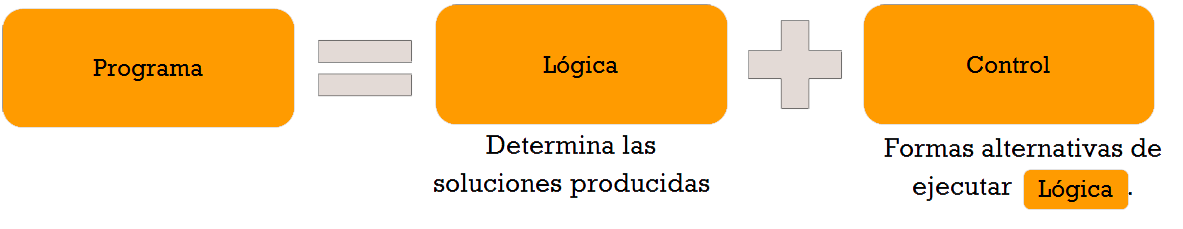
\includegraphics[width=14cm]{./Imagenes/img02} 
\end{center}

Asume que partimos de un conjunto de hechos y reglas conocidos. Solamente es la declaración del componente lógico de un algoritmo. El sistema desarrolla el componente de control de secuencia. En este paradigma, la evaluación asume que cuando se selecciona una regla, es porque ésta es la única posibilidad o la necesaria para resolver el problema. Es decir, se encuentra una solución si un conjunto de reglas adecuado y las sustituciones a dichas reglas producen un conjunto de reglas aterrizadas (sin variables libres), suficientes para deducir el resultado de los hechos conocidos.
La programación lógica intenta resolver lo siguiente:
Dado un problema S, saber si la afirmación A es solución o no del problema o en que casos lo es. Además queremos que los métodos sean implantados en maquinas de forma que la resolución del problema se haga de forma automática
La programación lógica: construye base de conocimientos mediante reglas y hechos.

\textbf{Características}\\
\begin {itemize}
\item Los programas para los lenguajes de programación lógicos son un conjunto de hechos y reglas.
\item La sintaxis de los lenguajes de programación lógicos es notablemente diferente de los lenguajes de programación imperativos.
\item Unificación de términos.
\item Mecanismos de inferencia automática.
\item Recursión como estructura de control básica.
\item Visión lógica de la computación.
\item La aplicación de las reglas de la lógica para inferir conclusiones a partir de datos.
\item El programa se transforma en un conjunto de declaraciones formales de especificaciones que deben ser correctas por definición.
\item No tiene un algoritmo que indique los pasos que detallen la manera de llegar a un resultado.
\item Las salidas son funcionalmente dependientes de las entradas.

\textbf{Ventajas y Desventajas del uso de este paradigma}
\textbf{Ventajas}
\item Puede mejorarse la eficiencia modificando el componente de control sin tener que modificar la lógica del algoritmo.
\item Relaciones multipropósito.
\item Simplicidad.
\item Generación rápida de prototipos e ideas complejas.
\item Sencillez en la implementación de estructuras complejas.
\item Potencia.

\textbf{Desventajas}
\item Altamente ineficiente.
\item Pocas áreas de aplicación
\item No existen herramientas de depuración efectivas.
\item En problemas reales, es poco utilizado.
\item Si el programa no contiene suficiente información para contestar una consulta responde false.	

\end{enumerate}

\section{Paradigma No 04 – Programación Funcional} 

\begin{enumerate}[1.]
	\item La Programación Funcional  es una forma en la cual podemos resolver diferentes problemáticas ya que estaremos trabajando principalmente con funciones, evitaremos los datos mutables, así como el hecho de compartir estados entre funciones.
	
\begin{center}
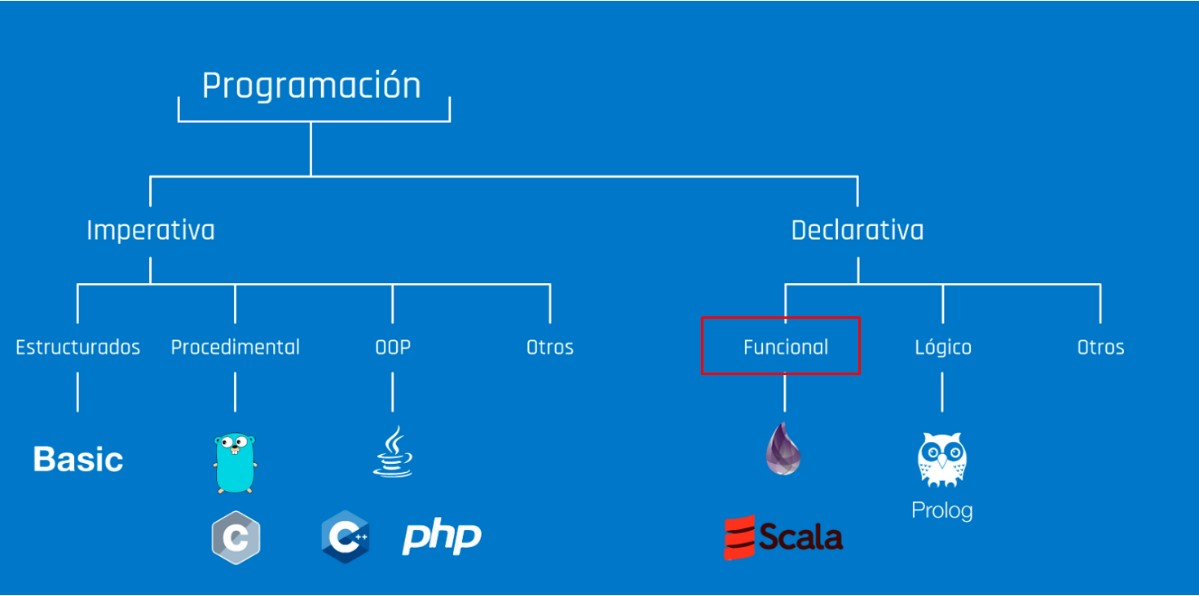
\includegraphics[width=14cm]{./Imagenes/img04} 
\end{center}

	\\Las funciones serán tratadas como ciudadanos de primera clase. Las funciones podrán ser asignadas a variables además podrán ser utilizadas como entrada y salida de otras funciones.
	
\emph{Ejemplo:}

De forma tradicional imperativa tendríamos que especificar “como” lo haremos
\begin{center}
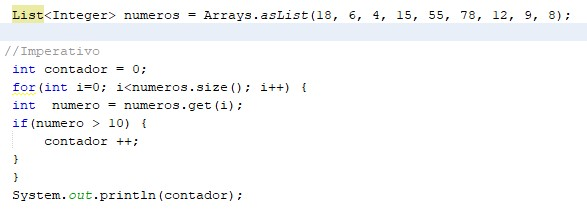
\includegraphics[width=14cm]{./Imagenes/img05} 
\end{center}

Pero de forma declarativa o programación funcional tendríamos: 

\begin{center}
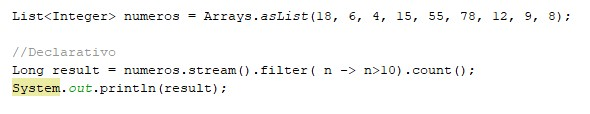
\includegraphics[width=14cm]{./Imagenes/img06} 
\end{center}
 
\end{enumerate}

\section{Paradigma No 05 – Principios de Diseño de Base de Datos} 

\begin{enumerate}[1.]
	\item Uno de los pasos cruciales en la construcción de una aplicación que maneje una base de datos, es sin duda, el diseño de la base de datos. Si las tablas no son definidas apropiadamente, podemos tener muchos dolores de cabeza al momento de ejecutar consultas a la base de datos para tratar de obtener algún tipo de información.
	\\No importa si nuestra base de datos tiene sólo 20 registros, o algunos cuantos miles, es importante asegurarnos que nuestra base de datos está correctamente diseñada para que tenga eficiencia y usabilidad a lo largo del tiempo.

\\En este artículo, se mencionarán algunos principios básicos del diseño de base de datos y se tratarán algunas reglas que se deben seguir cuando se crean bases de datos. Dependiendo de los requerimientos de la base de datos, el diseño puede ser algo complejo, pero con algunas reglas simples que tengamos en la cabeza será mucho más fácil crear una base de datos perfecta para nuestro siguiente proyecto.

\\Construir grandes aplicaciones en MySQL resulta fácil con herramientas como Apache, Perl, PHP, y Python. Asegurarse de que son rápidas, sin embargo, requiere algo más que perspicacia. MySQL tiene una bien merecida reputación de ser un servidor de bases de datos muy rápido que también es muy fácil de configurar y usar, además de que en los últimos años su popularidad ha crecido notablemente debido a que se utiliza en infinidad de sitios web que requieren hacer uso de una base de datos. Sin embargo, pocos usuarios sabemos algo más que crear una base de datos y escribir algunas búsquedas contra ella.

\\Después de leer este artículo debemos ser capaces de entender algunas técnicas que nos ayudarán a diseñar bases de datos MySQL para construir mejores aplicaciones. Vamos a suponer que se tiene un conocimiento básico del lenguaje SQL, y de MySQL, pero no vamos a asumir que se tiene mucha experiencia en alguno de los dos.
	

\end{enumerate}

\section{CONCLUSIONES} 

\begin{enumerate}[1.]
	\item La programación funcional nos permitirá desarrollar software mucho más legible y fácil de testear, nos concentramos en qué estamos haciendo y no en cómo.
	\\Aunque a primera vista pueda parecer que este tipo de programación está muy limitada a resolver puzzles y cosas por el estilo, lo cierto es que (teóricamente) puedes realizar cualquier tipo de programa con ellos.

Aun así, lo lógico (valga la redundacia) es utilizar programación lógica en las áreas en que más sentido tiene: inteligencia artificial, sistemas expertos, procesamiento de lenguajes, etc.

El poder utilizar este paradigma a través de librerías hace sea mucho más atractivo, porque hace que sea más sencillo usarlo sólo en aquellas partes del problema que tiene sentido.
	

\end{enumerate}
